\section{Realization of a General Three-Qubit Quantum Gate}
\subsection{Two-Qubit Quantum Gates Recap}
\begin{frame}
\frametitle{Two-Qubit Quantum Gates Recap}
\begin{figure}
  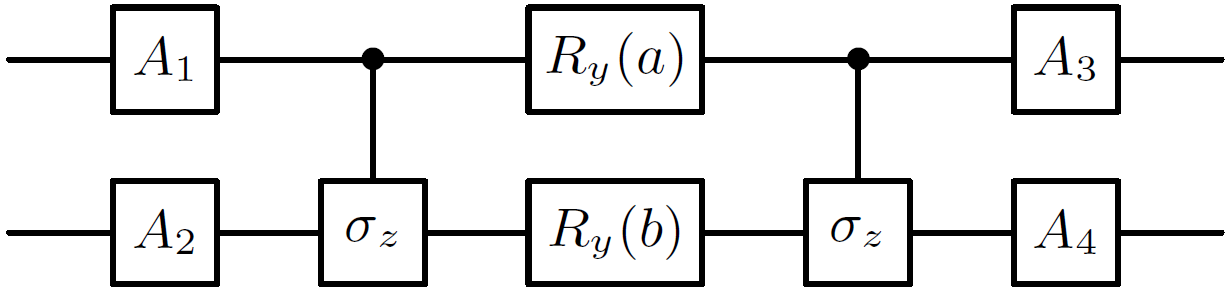
\includegraphics[width=\textwidth]{figure/two-qubit.png}
  \caption{Optimal Quantum Circuits for General Two-Qubit Gates are 15 single qubit gates and 3 CNOT gates\cite{two}}
\end{figure}
\end{frame}

\subsection{Introduction to Three-Qubit Quantum Gates}
\begin{frame}
\frametitle{Realization of Three-Qubit Quantum Gates}
\begin{itemize}
  \item universal gate family: $\{R_z,R_y,CNOT\}$
  \item basic idea: KAK Algorithm\cite{kak}, block-diagonal matrix
  \item results:98 single qubits and 40 CNOT gates
\end{itemize}
% introduce three qubit gates and the tools
\end{frame}

\subsection{Realization Techniques}
\subsubsection{Decomposition}
\begin{frame}
\frametitle{KAK Decomposition\cite{kak}}
any $SU(8)$ can be decomposed as
\begin{align}
  U&=K_{1} \exp \left(-i\left(\beta_{1} XXX+\beta_{2} YYX+\beta_{3} ZZX+\beta_{4} IIX\right)\right) K_{2}\\
  K_{1}&= P_{1}\exp \left(-i\left(\alpha_{1}XXX + \alpha_{2}YYZ + \alpha_{3}ZZZ\right)\right)P_{2},\\
  K_{1}&= P_{3}\exp \left(-i\left(\gamma_{1}XXX + \gamma_{2}YYZ + \gamma_{3}ZZZ\right)\right)P_{4}
\end{align}
% AKA results and step followed
\end{frame}
\begin{frame}
\frametitle{KAK Decomposition\cite{kak}}
\begin{figure}
  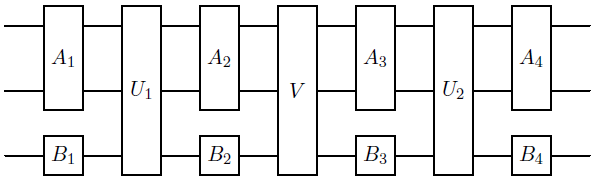
\includegraphics[width=.8\textwidth]{figure/three.png}
  \caption{KAK decomposition of a three-qubit unitary operation.}
\end{figure}
% AKA results and step followed
\end{frame}
\subsubsection{Diagonalization}
\begin{frame}
\frametitle{Diagonalization}
\begin{itemize}
  \item target:
  \begin{align}
    P=&\begin{bmatrix}
      P_1 &&\\
      &P_1 &&\\
      &&P_2&\\
      &&&P_2
    \end{bmatrix}
    ,\\P_{1}=\begin{bmatrix}
        \cos (a-b) & i \sin (a-b) \\
        i \sin (a-b) & \cos (a-b)
        \end{bmatrix} \quad &\text { and } \quad 
        P_{2}=\begin{bmatrix}
        \cos (a+b) & i \sin (a+b) \\
        i \sin (a+b) & \cos (a+b)
        \end{bmatrix}
  \end{align}
  % figure need of use matrix
  \item using $\{CNOT,CZ,SWAP\}$
\end{itemize}
% how and results figure
\end{frame}
\subsubsection{Block-Diagonalization}
\begin{frame}
\frametitle{Block-Diagonalization}
\begin{figure}
  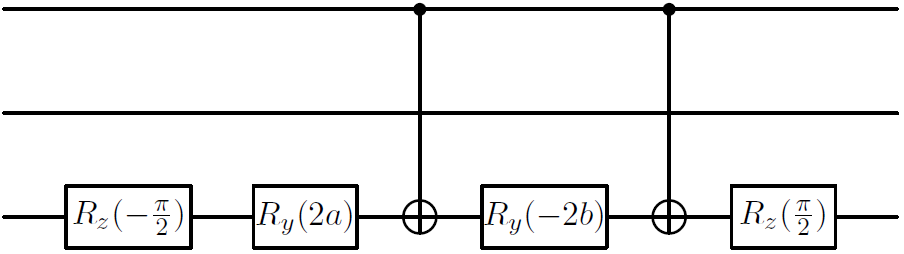
\includegraphics[width = .8\textwidth]{figure/P.png}
  \caption{a realization of Block-Diagonalization P}
\end{figure}
% result and way
\end{frame}
\begin{frame}
  \frametitle{Diagonalization}
  \begin{figure}
    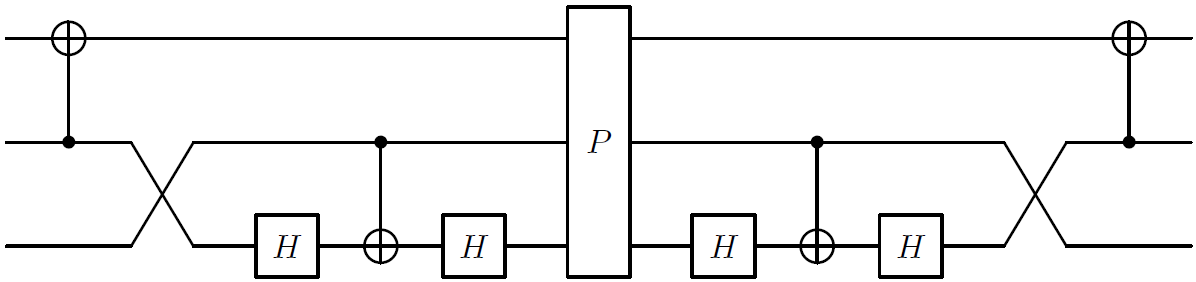
\includegraphics[width=.8\textwidth]{figure/N1.png}
    \caption{Decomposition of the unitary operation$\exp(i(a XXZ+b YYZ))$}
  \end{figure}

  \begin{figure}
    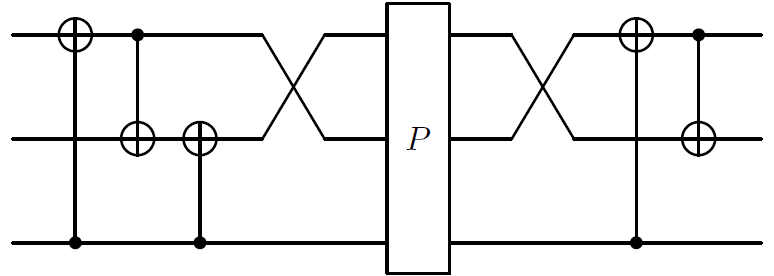
\includegraphics[width=.5\textwidth]{figure/M1.png}
    \caption{Decomposition of the unitary operation $\exp(i(\alpha_1 XXX+\alpha_2 YYX))$}
  \end{figure}
\end{frame}

\begin{frame}
  \frametitle{whole circuit}
  \begin{figure}
    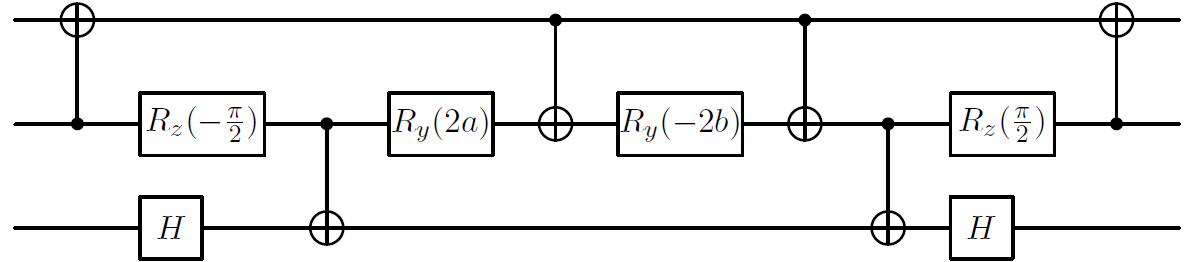
\includegraphics[width = .8\textwidth]{figure/N1wole.png}
    \caption{a realization of Block-Diagonalization P}
  \end{figure}
  \begin{figure}
    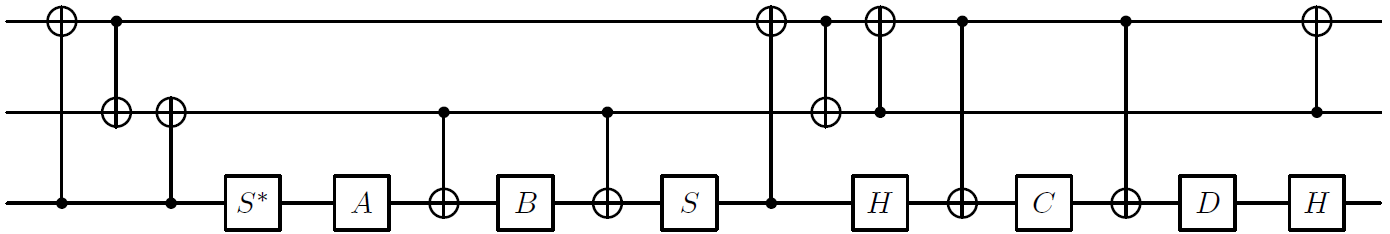
\includegraphics[width = .8\textwidth]{figure/M.png}
    \caption{a realization of Block-Diagonalization P}
  \end{figure}
\end{frame}
\subsubsection{Count}
\begin{frame}
\frametitle{Count}
  \begin{figure}
    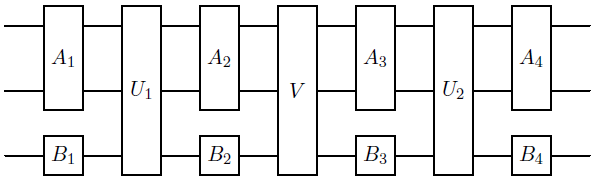
\includegraphics[width=.8\textwidth]{figure/three.png}
  \end{figure}
  \begin{align}
    &9\times 2+10 +3\times 4=40\\
    &5\times 2 +6+ 15\times4+3\times 4=88
  \end{align}
%  the whole number
\end{frame}
